
\chapter{相关工作与国内外研究现状}
\label{chapter:relate}

\section{文本匹配研究现状}

文本匹配是自然语言处理的一个基础问题。传统的文本匹配算法往往是基于向量空间模型进行的,往往在词汇级别匹配的基础上辅助以各种规则进行处理。这导致整体算法逻辑策略复杂,难以解决语义层面的匹配问题。

近年来,随着计算机计算能力的不断提升,互联网数据的爆炸增长,深度学习相关的算法获得了巨大的发展并开始广泛的应用于图像识别、文本处理等等领域。因此自然而然的,开始有学者试图利用深度学习解决文本匹配问题。

\subsection{基于单文档语义表达的深度匹配模型}
单文档语义表达匹配是将每个文档表示为低维向量,通过计算向量相似度得到两者的匹配程度。
\begin{figure}[!htbp]\centering
  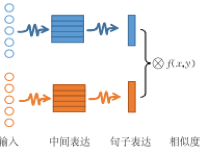
\includegraphics[width=0.4\linewidth]{match_single_doc.png}
  \caption{单文档语义表达匹配框架}{text match based on single document semantics}
  \label{fig:text match based on single document semantics}       % Give a unique label
\end{figure}

深度语义结构模型\cite{Huang2013LearningDS}是最早利用深度学习进行文本匹配的工作,主要是针对查询和文档的匹配任务。它通过搜索引擎里查询和文档的点击日志,利用深度网络得到查询和文档的向量表示,通过余弦相似度计算两个句子的语义相似度,最终得到相似度模型。

深度语义结构模型主要分成3层:输入、表示和匹配层。输入层上对于引文的处理方式为词哈希(word hashing),将每个英文单词切分成 3 个字母为一组的单词。这样可以压缩空间。增强泛化能力;中文以单字的一位有效编码(one-hot)进行输入。在表示层,采用词袋(Bag of words)的方式,输入一个 4 层神经网络,输出 128 维的向量表示,匹配层使用 softmax 进行分类预测。

\begin{figure}[!htbp]\centering
  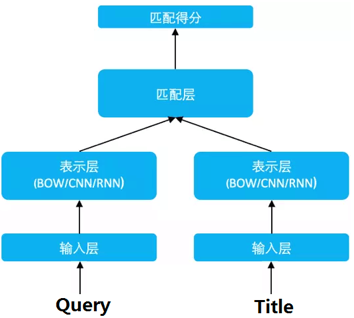
\includegraphics[width=0.8\linewidth]{DSSM.png}
  \caption{深度语义结构模型}{DSSM model}
  \label{fig:DSSM}       % Give a unique label
\end{figure}

这种方法可以减少对切词算法的依赖,提高模型的泛化能力。但是由于使用词袋模型,丧失了语序信息和上下文信息,而且全连接的神经网络参数过多,难以训练。
针对于上面的问题,微软提出了基于单词序列的卷积深度语义模型(CLSM)\cite{Shen2014ALS}。与 DSSM 相比,CLSM 主要对输入和表示层进行了改进。
在输入层上,CLSM加入了一个滑动窗口,利用滑动窗口提取序列信息。

\begin{figure}[!htbp]\centering
  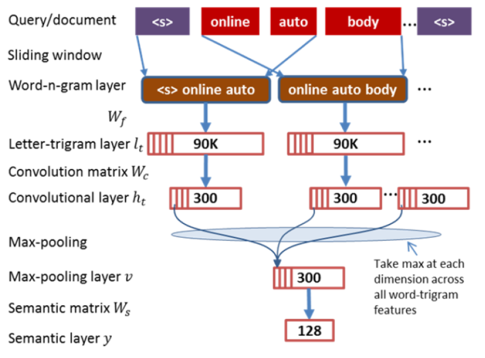
\includegraphics[width=0.8\linewidth]{CLSM.png}
  \caption{CLSM结构模型}{CLSM model}
  \label{fig:CLSM}       % Give a unique label
\end{figure}

在 \ref{fig:CLSM} 的结构中,我们可以看到选择的滑动窗口大小为3。对于一个滑动窗口内的词,类似DSSM,它将每个单词的3-字母组合的词哈希向量相加得到最终的向量表示。原模型中所使用的数据集最终被映射为 9 万维的向量。在表示层上,我们可以看到模型使用了卷积神经网络,利用卷积层的特征进行上下文的特征提取,利用池化层发现全局的上下文特征,最后你这个利用全连接层将提取到的特征进行压缩得到了 128 维的句子的向量表达。

相对于DSSM,CLSM 通过卷积和池化提取全局的上下文信息,但是对于间隔较远的上下文信息,由于卷积神经网络的限制仍然难以捕捉。
针对于这种问题,有人想到利用 LSTM 建模上下文信息,提出了LSTM-DSSM\cite{Palangi2014SemanticMW},整体的网络结构为:

\begin{figure}[!htbp]\centering
  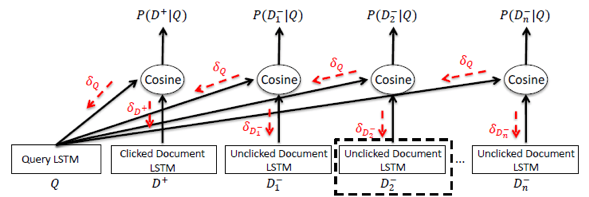
\includegraphics[width=0.8\linewidth]{LSTM-DSSM.png}
  \caption{LSTM-DSSM结构模型}{LSTM-DSSM model}
  \label{fig:LSTM-DSSM}       % Give a unique label
\end{figure}

相对于CLSM,LSTM-DSSM主要是将 CNN 换成了 LSTM。

\subsection{直接建模匹配的深度匹配模型}
直接建模匹配的模型直接对匹配问题进行建模,提取相应的特征。这种方式更加直观,也更符合人类判断两个句子是否相似的过程。

MatchPyramid\cite{Pang2016TextMA}利用匹配矩阵建模两个句子的交互过程。匹配矩阵中每个值都是2个句子中词两两计算得到的相似度。相似度可以使用词向量的余弦相似度或点积等进行刻画,而2个词在各自句子中的位置自然组成了一个二维坐标,因此构造出了匹配矩阵。之后将匹配的问题建模为在这个矩阵上进行图像识别的过程,利用卷积和池化操作捕捉局部和全局的交互信息。

\begin{figure}[!htbp]\centering
  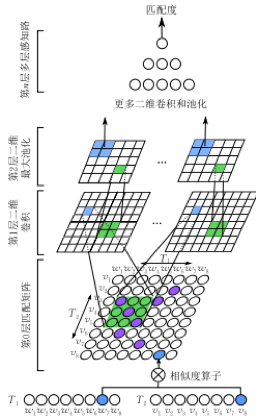
\includegraphics[width=0.4\linewidth]{MatchPramid.png}
  \caption{MatchPramid 模型}{MatchPramid model}
  \label{fig:MatchPramid}       % Give a unique label
\end{figure}

\section{强化学习研究现状}
\label{sec:rl_intro}
强化学习\cite{Sutton1998ReinforcementL}是机器学习中的一个重要研究领域,它以试错的机制与环境(Environment)进行交互,通过最大化累积奖赏来学习最优策略。强化学习研究的问题往往有三个特征:闭环性,学习系统产生的行为(action)会影响后续输出;无监督,学习对象只能通过学习得到行为的信息;行动产生的结果,包括奖励(reward),会影响较长时间。

一个强化学习过程可以被定义为一个五元组<$S, A, P, R, \pi$>,其中:
\begin{itemize}
  \item[•] 状态(Status,S)是环境的状态;
  \item[•] 动作(Action, A)是主体在特定环境下使用的策略
  \item[•] 转移概率(Transition function,P)是环境受主体动作影响后状态的迁移概率;
  \item[•] 奖励(Reward,R)是环境根据主体行为返回给主体的信号,主体根据奖励调整自己的策略;
  \item[•] 策略(Policy,$\pi$)定义了特定环境下主体的行为方式,表示状态到动作的映射关系。策略分为确定性和随机性两种。
\end{itemize}

\begin{figure}[!htbp]\centering
  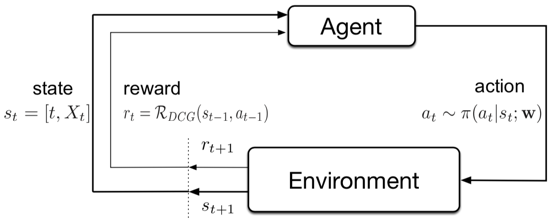
\includegraphics[width=0.7\linewidth]{interaction.png}
  \caption{主体与环境的交互}{interaction between agent and enviroment}
  \label{fig:interaction}       % Give a unique label
\end{figure}

主体和环境的交互可以用图\ref{fig:interaction}表示。主体在当前状态$s_t$下根据策略π选择动作$a_t$,环境接收到该动作并转移到下一状态$s_{t+1}$,主体接收环境反馈回来的奖励选择下一步动作。强化学习不需要监督信号,主要算法包括Q学习(Q-learning),策略梯度(policy gradient)等等。

深度强化学习的主要思路是将神经网络用于复杂高维数据的特征提取,转化到低维特征空间便于强化学习处理。
由于卷积神经网络对图像处理拥有天然的优势,将卷积神经网络与强化学习结合成了研究热点。
2013年,DeepMind团队提出了深度Q网络(DeepQ Network,DQN)\cite{Mnih2013PlayingAW}并将该网络应用于Atari视频游戏,首次在复杂高维的状态空间下使用深度强化学习学会了游戏策略。

2015年,DeepMind团队进一步完善了DQN算法\cite{Mnih2015HumanlevelCT}。
DQN将深度卷积神经网络和Q学习结合到一起,并集成了经验回放技术(memory reply)和目标Q网络。
经验回放通过周期采样历史数据增加了数据的利用效率,同时减少了数据之间的相关性。
DQN在大部分Atari视频游戏中实现了人类玩家的控制效果,是深度强化学习领域重要的开创性工作。

2016年初,DeepMind团队发表了围棋AI:AlphaGo\cite{Silver2016MasteringTG}。AlphaGo 的问世将深度强化学习的研究推向了新的高度。它创新性地结合深度强化学习和蒙特卡罗树搜索,通过策略网络选择落子位置降低搜索宽度,使用价值网络评估局面以减小搜索深度,这样搜索效率得到了大幅提升,胜率估算也更加精确。与此同时,AlphaGo 使用强化学习的自我博弈来对策略网络进行学习,改善策略网络的性能,使用自我对弈和快速走子结合形成的棋谱数据进一步训练价值网络。最后在在线对弈时结合策略网络和价值网络的蒙特卡罗树搜索在当前局面下选择最终的落子位置。

\begin{figure}[!htbp]\centering
  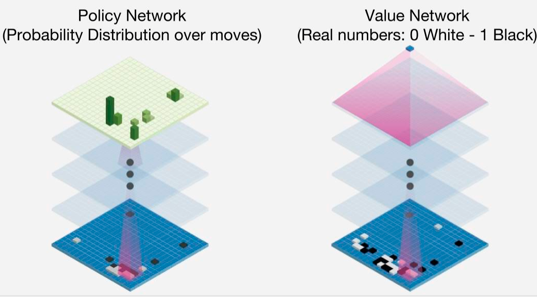
\includegraphics[width=0.8\linewidth]{AlphaGo.png}
  \caption{AlphaGo的策略网络和价值网络} {AlphaGo policy and value network}
  \label{fig:AlphaGo}       % Give a unique label
\end{figure}

2017年初,AlphaGo Zero\cite{Silver2017MasteringTG}对AlphaGo进行了改进和升级。它将策略网络和价值网络整合在一起,直接利用深度强化学习方法进行端到端的自我对弈学习。
相比于 AlphaGo,AlphaGo Zero 不需要任何先验知识,只要将棋局作为输入即可;策略网络和价值网络的整合使得神经网络的复杂度降低,因此降低了硬件的资源需求,减少了训练时间。

AlphaGo Zero的成功证明了在没有任何先验经验的情况下,深度强化学习在围棋领域仍然能取得巨大的成功;而在围棋下法上,AlphaGo Zero创造了更多的下棋方式,大大开拓了人类对围棋的认知。
虽然基于蒙特卡罗树搜索的深度强化学习方案已经取得了成功,但是由于搜索算法带来的时间和空间开销,使得其很难满足实时性的需求。目前强化学习很难在星际争霸这种实时游戏上战胜人类。

\begin{figure}[!htbp]\centering
  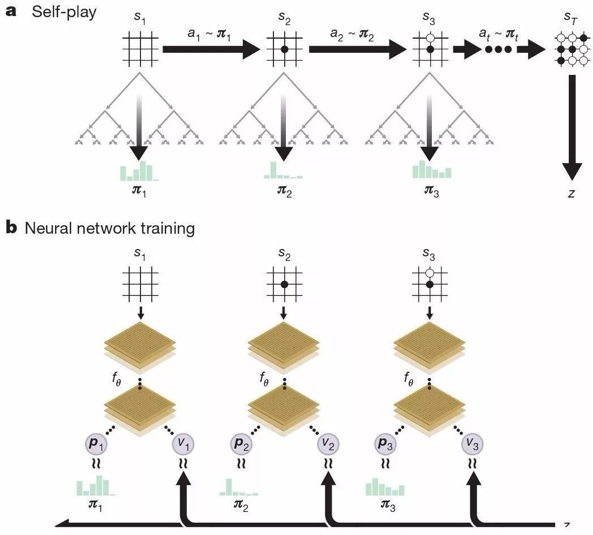
\includegraphics[width=0.8\linewidth]{AlphaGo_Zero.png}
  \caption{AlphaGo Zero 自我对弈训练过程} {training process of AlphaGo Zero}
  \label{fig:AlphaGo_Zero}       % Give a unique label
\end{figure}

\section{本章小结}

本章主要介绍了文本匹配和强化学习的相关工作与研究现状。

近年来,深度学习开始广泛利用于文本匹配任务中。目前基于深度学习的文本匹配算法都试图利用神经网络理解输入句子的语义信息,主要分为对基于单文档的语义理解以及直接对匹配过程进行建模。对单文档的语义理解利用神经网络抽取出每个句子的语义向量,组合后通过计算得到最后的输出;直接建模匹配过程利用匹配矩阵通过卷积或者循环网络的方式建模局部和全局的交互信息。

强化学习近年来获得了长足的发展。在利用强化学习解决游戏问题上,学者对传统的 policy gradient 和 value iteration 进行了改进,先后提出了 DQN,AlphaGo,AlphaGo Zero 等算法,并在 Atari,围棋等领域取得了极大的成功。
